% Paper 3 body. Every number is a macro from generated/p3_macros.tex or a table from generated/, written by
% figs/make_figures.py from results/paper3.

\section{Introduction}\label{sec:intro}

A world model for retail earns its keep on the plans a merchant has not yet run. Forecasting next week under the
plan already agreed is something gradient-boosted trees do well; the reason to carry each item's state under the
plan, as a world model does, is to ask what a different plan would bring: a deeper cut, a new regular price, a
promotion in a quiet week. Our forecasting study~\cite{rwm} compared world models with trees and foundation models
on the plans merchants made. That comparison cannot say whether the model is right about plans nobody made, because
real data hold no answer for them.

This paper measures it. In generated stores where the expected sales of any plan are known~\cite{paper2}, we train
models on the plans merchants make and ask them to forecast plans held out by design. We find:

\begin{itemize}\setlength{\itemsep}{1pt}
\item \textbf{Forecast accuracy is a fair guide between kinds of model, and a poor one between versions of a world
model.} Across all 25 versions in each world, better forecasters simulate new plans better (\linkAllMin{} to
\linkAllMax{}, every interval above zero). Within the world model's versions, where plans follow demand, the link
reverses (\linkBWmOne{}, \linkBWmOneCi{}).
\item \textbf{Training the world model to learn actions does not fix it.} JEPA pretraining, a latent consistency
check, a check seven weeks ahead and adaptation at the plan date move its error on new plans by at most 0.05.
\item \textbf{A world model with the shape of the price response built in does.} Its error on new plans is
\errBShape{} in the world whose response bends, against \errBWm{} for the plain world model, \errBLgb{} for LightGBM
and \errBLlRr{} for a log-linear model given the recorded regular price, and it forecasts the merchants' own plans
at least as well (\fcBShape{} against \fcBWm{}).
\item \textbf{The recorded regular price is the input that matters most.} Without it every model reads a lasting
price move as a temporary cut; with it the log-linear model's error falls from \errLLl{} to \errLLlRr{} in the world
that matches its form.
\end{itemize}

The rest of the paper sets out the stores (\S\ref{sec:data}), the models and remedies (\S\ref{sec:method}), the
setup (\S\ref{sec:setup}) and the results (\S\ref{sec:results}). The plan for this study was fixed before any run,
and both amendments were written before the runs they added (Appendix~\ref{app:plan}).

\section{Related work}\label{sec:related}

\paragraph{World models} Learned models of how an environment responds to actions are used to plan in games and
control~\cite{worldmodels,planet,dreamerv3,tdmpc2}. Joint-embedding predictive architectures learn such models by
predicting in a latent space rather than in the raw signal~\cite{lecun2022,ijepa,vjepa2,leworldmodel}; recent work
separates the effect of the action from the drift of the world~\cite{dwm} and trains the model to tell actions
apart~\cite{adwm}. Our molecular work found that predictive pretraining transfers to scaffolds not seen in
training~\cite{mjepa}. We test whether these training choices make a retail world model right about plans outside
its history, and find they do not on their own.

\paragraph{Retail promotion and price models} Log-linear models of sales on price, promotion and display have long
been the retailer's tool for promotion planning~\cite{promocast,vanheerde2000,vanheerde2003}, with well-studied
elasticities~\cite{hoch1995,bijmolt2005}. Machine-learning forecasters now lead on accuracy~\cite{m5accuracy,
fildes2022,ma2016}. We use the log-linear model as the reference a world model has to beat on plans, and show where
its fixed form fails.

\paragraph{Extrapolation and structure} Models fitted to logged decisions are unreliable for actions the logging
policy rarely took~\cite{levine2020,pearl2009}, and models with equal held-out accuracy can behave very differently
off the data~\cite{damour2022}. Monotone networks~\cite{sill1998,you2017} and physics-informed models~\cite{
karniadakis2021} build known structure into a learned model so it extrapolates sensibly. We bring that idea to the
price response of a retail world model.

\paragraph{Our own studies} The forecasting study~\cite{rwm} measures accuracy on observed plans on four public data
sets; the explanation audit~\cite{paper2} tests whether a model's stated lift is right. This paper reuses no result
of either: its worlds use new seeds, two new world shapes and new held-out plans, and its measures are new.

\section{Generated stores with known answers}\label{sec:data}

Each world has 18 stores in three price zones and 20 items over 260 weeks. Weekly sales are Poisson around an
expected level set by the item's size, the season, a persistent demand shock and the plan: the price (a temporary
cut below the regular price), a promotion, a display, the week after a planned week, and the regular price itself.
The truth for any plan is the expected level the generator gives it, so the effect of a plan never run is known
exactly.

\paragraph{Planning into demand} Merchants plan cuts and promotions into weeks they expect to be strong. A
planning strength of 0 places plans at random; strengths 0.5, 1 and 1.5 tie them more closely to the demand shock,
so a model that reads the plan as the cause of high sales overstates its effect.

\paragraph{Two shapes of world} In the \emph{log-linear world} a cut of depth $c$ multiplies sales by
$(1-c)^{-2.5}$ and the regular price acts with elasticity $-0.5$; this is the form of the log-linear model, which
therefore matches the truth by construction. In the \emph{bent world} the gain from a cut flattens,
$1 + 1.015\,(1 - e^{-c/0.15})$ (equal to the log-linear world at a 20\% cut), the regular-price response is linear
in the price ratio, and a promotion with a display adds less than both alone. Each shape is generated at four
planning strengths and three seeds: 24 worlds.

\paragraph{Test and learn} A further 24 worlds add random test plans: 5\% of training item-weeks get a cut of 10\%
to 40\% (the merchants' own range), a promotion and a display, each with probability one half, placed apart from
demand. The tests come from their own random stream, so everything else in the world is unchanged. The cuts stay
inside the range merchants use, so the deeper cuts held out below remain unseen.

\section{Models and remedies}\label{sec:method}

\paragraph{World model} The state model of our forecasting study~\cite{rwm}: an encoder reads each item's last 13
or 26 weeks of sales and plan into a state, a recurrent cell rolls the state forward under the plan, and a readout
gives expected sales as a baseline times a lift. Twelve versions per world vary the width (16, 32, 64), training
steps (500, 2{,}000) and history (13, 26 weeks).

\paragraph{LightGBM} Gradient-boosted trees~\cite{lightgbm} with the plan as features, one model per horizon week.
Twelve versions vary the leaves (7, 31, 127), rounds (100, 500) and minimum rows per leaf (20, 100).

\paragraph{Log-linear model} Poisson regression of sales on the series, season, log price over the regular price,
log regular price over the series' mean, promotion, display, both together and the week after a planned week. The
regular price is the highest price of the last 12 weeks, as for the other models.

\paragraph{Remedies added after the first results} Each changes one thing and is given to every model it applies
to on the same data.
\begin{enumerate}\setlength{\itemsep}{1pt}
\item \emph{Learning actions}: JEPA pretraining (500 steps on the latent loss first), the latent consistency check,
the check seven weeks ahead, and adaptation at the plan date.
\item \emph{The recorded regular price}: retailers know whether a price is a cut or a new regular price. Every
model is given it (versions marked ``+ recorded regular price'').
\item \emph{Split the job}: the forecaster gives the week at the current regular price with nothing planned; the
log-linear model with the recorded regular price gives the change the plan makes.
\item \emph{World model with a price shape}: the plan's price reaches the world model only through
\begin{equation}\label{eq:shape}
\log m = a_1\bigl(1 - e^{-c/b}\bigr) - a_2 \log(1-c) - \gamma \log\frac{r}{\bar p},
\end{equation}
where $c$ is the cut (capped at 95\%), $r$ the recorded regular price, $\bar p$ the item's usual price, and
$a_1, a_2, b, \gamma > 0$ are learned per item and store from their labels. Sales cannot fall as a cut deepens. The
first term flattens at $a_1$; the second grows without limit as the cut nears 100\% and is held finite only by the
cap on the cut, so the model learns from the data how far the gain keeps rising. A lasting regular price acts
through its own elasticity. The rest of the network sees
neither price, so it cannot learn a price effect that breaks these rules.
\item \emph{Test and learn}: every model refitted on the worlds with random test plans.
\end{enumerate}

\section{Experimental setup}\label{sec:setup}

Models are fitted on weeks 1 to 252 and forecast weeks 253 to 260 from the same origin, under the merchants' own
plan and under eight held-out plans: every planned cut deepened to 50\% and to 60\% (training cuts run from 10\% to
40\%); the regular price moved 10\% and 5\% down and up for the whole horizon; promotions and displays moved to each
series' lowest-demand weeks; and no plan.

\paragraph{Measures} \emph{Forecast accuracy}: item-by-store RMSSE on the merchants' own plan. \emph{Error on new
plans}: for each held-out plan, the predicted change in sales (held-out plan minus own plan, summed) over the true
change; the error is $|\log|$ of that ratio, 0 when the change is right, capped at a twentyfold miss, which a wrong
sign also counts as; we report the mean over the eight plans. \emph{Decisions}: the revenue given up by the
regular-price move (of $-10\%, -5\%, 0, +5\%, +10\%$) the model picks; the true lift missed by switching on the
promotions with the largest predicted lift in half the item-weeks; and the error of ordering stock to the forecast.

\paragraph{The test} Within each world, the rank correlation over the 25 versions between forecast error and each
measure, averaged over three seeds, with a 95\% interval from 2{,}000 bootstrap draws of versions. The same
correlation within each model class was added after the first results.

\section{Results}\label{sec:results}

\subsection{Better forecasting is a fair guide between kinds of model, not between versions}

Across all 25 versions, the models that forecast the merchants' plans better also simulate new plans better, in
every world (Table~\ref{tab:link}; Figure~\ref{fig:link}b,c): \linkLAllLo{} to \linkLAllHi{} in the log-linear
world and \linkBAllLo{} to \linkBAllHi{} in the bent world, every interval above zero. The link comes mostly from
the gap between kinds of model: LightGBM forecasts and simulates better than the plain world model
(Figure~\ref{fig:link}a).

Within the world model's own versions the link depends on how merchants plan. With plans placed at random it holds
(\linkLWmZero{} and \linkBWmZero{}). Where plans follow demand it reverses: \linkBWmOne{} (\linkBWmOneCi{}) in the
bent world and \linkLWmOneHalf{} (\linkLWmOneHalfCi{}) in the log-linear world at the strongest planning. The
versions that forecast best are those that learn most from the merchants' plans, and where plans follow demand
those plans teach the wrong effect. Choosing a world model version on forecast accuracy can choose the worst
simulator. Stock error tracks forecast accuracy closely in every class (Table~\ref{tab:link}), as ordering to a
forecast should.

\begin{table*}[t]
\centering
\caption{\textbf{Does better forecasting go with better simulation?} Rank correlation, within each world, between
forecast error on the merchants' plans and each measure (higher is worse for every measure, so a positive number
means better forecasters are also better at it), averaged over three seeds. Bold: the 95\% bootstrap interval excludes
zero. --: every version made the same choice, so there is nothing to rank. All versions: the test fixed in the plan (12 world model, 12 LightGBM and the log-linear model). Within a model
class: added after the first results.}
\label{tab:link}
\footnotesize\setlength{\tabcolsep}{4pt}
\begin{adjustbox}{max width=\textwidth}
\begin{tabular}{llrrrrrrrrr}
\toprule
 & & \multicolumn{3}{c}{All 25 versions} & \multicolumn{3}{c}{World model versions} & \multicolumn{3}{c}{LightGBM versions} \\
\cmidrule(lr){3-5}\cmidrule(lr){6-8}\cmidrule(lr){9-11}
World & Planning & New plans & Price choice & Stock & New plans & Price choice & Stock & New plans & Price choice & Stock \\
\midrule
Log-linear world & 0 & \textbf{0.51} & 0.15 & \textbf{0.32} & \textbf{0.64} & -- & \textbf{0.83} & 0.33 & \textbf{-0.44} & \textbf{0.88} \\
 & 0.5 & \textbf{0.33} & \textbf{0.44} & 0.14 & 0.18 & -- & \textbf{0.79} & 0.38 & -0.33 & \textbf{0.87} \\
 & 1 & \textbf{0.40} & 0.15 & 0.22 & -0.31 & -- & \textbf{0.67} & 0.23 & \textbf{-0.67} & \textbf{0.75} \\
 & 1.5 & \textbf{0.34} & 0.14 & \textbf{0.27} & \textbf{-0.35} & -- & \textbf{0.85} & 0.24 & \textbf{-0.74} & \textbf{0.87} \\
Bent world & 0 & \textbf{0.32} & 0.13 & \textbf{0.69} & \textbf{0.43} & \textbf{0.30} & \textbf{0.86} & 0.40 & \textbf{-0.36} & \textbf{0.84} \\
 & 0.5 & \textbf{0.54} & \textbf{0.55} & \textbf{0.84} & -0.25 & -- & \textbf{0.92} & 0.23 & -0.29 & \textbf{0.82} \\
 & 1 & \textbf{0.48} & \textbf{0.56} & \textbf{0.87} & \textbf{-0.69} & -- & \textbf{0.90} & 0.27 & \textbf{-0.44} & \textbf{0.89} \\
 & 1.5 & \textbf{0.66} & \textbf{0.46} & \textbf{0.89} & -0.05 & -- & \textbf{0.88} & \textbf{0.62} & \textbf{-0.52} & \textbf{0.91} \\
\bottomrule
\end{tabular}
\end{adjustbox}
\end{table*}


\begin{figure*}[t]
\centering
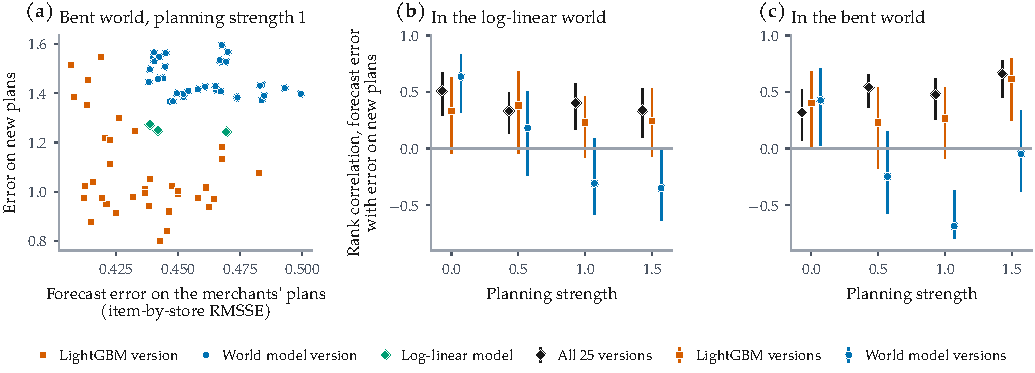
\includegraphics[width=\textwidth]{figs/fig_link.pdf}
\caption{\textbf{Forecast accuracy and error on new plans.} (a) Every version in the three bent worlds at planning
strength 1: forecast error on the merchants' plans against error on the held-out plans. (b, c) Rank correlation of
the two within each world, averaged over three seeds, with 95\% bootstrap intervals; all versions (the planned test)
and within each model class (added).}
\label{fig:link}
\end{figure*}

\subsection{Where the models go wrong}

Figure~\ref{fig:ratio} shows the predicted change over the true change for each held-out plan. Three failures stand
out. Every model without the recorded regular price reads a lasting regular-price move as a temporary cut: the
plain world model predicts \regdownLWm{} times the true gain from a 10\% lower regular price, LightGBM \regdownLLgb{}
times and the log-linear model \regdownLLl{} times, and each loses \priceLWm\%, \priceLLgb\% and \priceLLl\% of
revenue on the regular-price choice in the log-linear world. LightGBM cannot extend a response past the prices it
saw: it predicts \cutsixLLgb{} of the true gain from a 60\% cut. And the log-linear model extends its curve without
limit: in the bent world it predicts \cutsixBLl{} times the true gain from a 60\% cut.

\begin{figure*}[t]
\centering
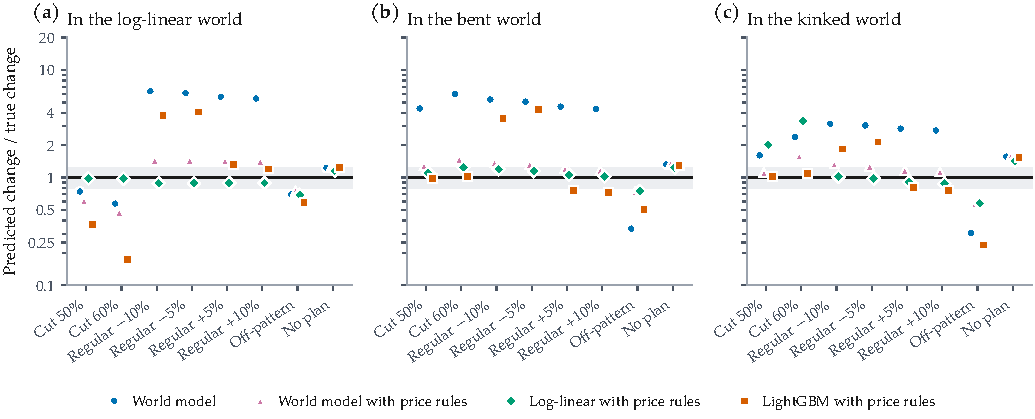
\includegraphics[width=\textwidth]{figs/fig_ratio.pdf}
\caption{\textbf{Predicted change in sales over the true change, for each held-out plan.} Medians over the 12 worlds
of each shape (planning strengths and seeds). 1 is right; the band marks 0.8 to 1.25. Log scale.}
\label{fig:ratio}
\end{figure*}

\subsection{Training the world model to learn actions does not help}

The four changes meant to make the world model learn the effect of actions leave its error on new plans where it
was: \errLActLo{} to \errLActHi{} against \errLWm{} in the log-linear world and \errBActLo{} to \errBActHi{}
against \errBWm{} in the bent world (Table~\ref{tab:remedies}, Figure~\ref{fig:remedies}). They change how the
state is learned; they do not change what the history contains, and the history holds no lasting price move
labelled as one and no cut deeper than 40\%.

\subsection{What works}

\paragraph{The recorded regular price} Given the recorded regular price, the log-linear model's error falls from
\errLLl{} to \errLLlRr{} in the log-linear world and from \errBLl{} to \errBLlRr{} in the bent world, and its
regular-price choice loses nothing. LightGBM gains little (\errLLgb{} to \errLLgbRr{}): trees cannot extend a
response beyond the regular prices seen. The plain world model given the regular price picks the right price move
but predicts almost no change in sales from it, so its error rises (\errLWmRr{}); a free network has no reason to
give the new input a sensible effect.

\paragraph{Split the job} The world model for the week with nothing planned and the log-linear model for the change
lowers the error to \errLSplit{} in the log-linear world, as good as the log-linear model alone, and to \errBSplit{}
in the bent world. It inherits the log-linear model's form, so in the bent world it overstates a 60\% cut
\cutsixBSplit{} times.

\paragraph{A world model with a price shape} Building the shape of Equation~\eqref{eq:shape} into the world model
gives the lowest error on new plans in the bent world, \errBShape{}, in all \worldsB{} worlds, against \errBSplit{}
for the split model and \errBLgb{} for LightGBM. It predicts \cutsixBShape{} times the true gain from a 60\% cut and
\regdownBShape{} times that of a 10\% lower regular price, loses \priceBShape\% on the price choice, and forecasts
the merchants' plans at least as well as any other model (\fcBShape{}). In the log-linear world it is second
(\errLShape{}) to the models that share the world's form (\errLLlRr{}): it learns too small a logarithmic term and understates the steep
gain of a 60\% cut there (\cutsixLShape{} of the truth). It is the only model with low error in both worlds.

\paragraph{Test and learn} Random test plans inside the merchants' range help every model a little: the shape model
from \errBShape{} to \tlShapeB{} and LightGBM from \errBLgb{} to \tlLgbB{} in the bent world; the plain world model
barely moves (\errBWm{} to \tlWmB{}). Tests break the link between plan and demand but cannot show a cut deeper
than the deepest tested; a model still needs a sensible shape to go beyond it.

\begin{figure*}[t]
\centering
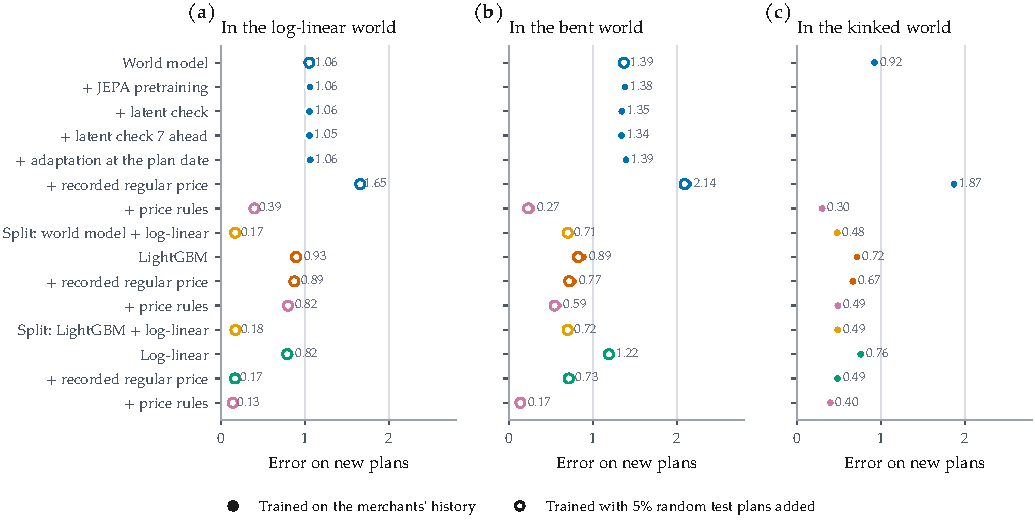
\includegraphics[width=\textwidth]{figs/fig_remedies.pdf}
\caption{\textbf{Error on new plans for every model and remedy} (0 means the predicted change in sales is right).
Medians over the 12 worlds of each shape. Filled: trained on the merchants' history; open: with 5\% random test
plans. Rows after the first in each block, and the split and shape rows, were added after the first results.}
\label{fig:remedies}
\end{figure*}

\begin{table*}[t]
\centering
\caption{\textbf{Every model and remedy in both worlds.} Medians over the 12 worlds of each kind (four planning
strengths, three seeds). Forecast: item-by-store RMSSE on the merchants' own plan in the held-out weeks. New plans:
mean over the eight held-out plans of $|\log(\text{predicted change}/\text{true change})|$. Price choice: revenue
given up by the regular-price move the model picks, \% of the best. Promotion choice: true lift missed by the
promotions the model picks, \% of the best. Stock: summed absolute error of ordering to the forecast, over expected
sales. Rows marked + change one thing in the row above them; all rows after the first in each model, and the split
and shape rows, were added after the first results (Appendix~\ref{app:plan}).}
\label{tab:remedies}
\footnotesize\setlength{\tabcolsep}{3.6pt}
\begin{adjustbox}{max width=\textwidth}
\begin{tabular}{lrrrrrrrrrr}
\toprule
 & \multicolumn{5}{c}{Log-linear world} & \multicolumn{5}{c}{Bent world} \\
\cmidrule(lr){2-6}\cmidrule(lr){7-11}
Model & Forecast & New plans & Price choice & Promotion & Stock & Forecast & New plans & Price choice & Promotion & Stock \\
\midrule
World model & 0.362 & 1.06 & 9.5 & 1.5 & 0.26 & 0.475 & 1.39 & 9.6 & 1.6 & 0.26 \\
\quad + JEPA pretraining & 0.364 & 1.06 & 9.5 & 1.6 & 0.26 & 0.471 & 1.38 & 9.6 & 1.4 & 0.26 \\
\quad + latent check & 0.364 & 1.06 & 9.5 & 1.7 & 0.26 & 0.469 & 1.35 & 9.6 & 1.6 & 0.25 \\
\quad + latent check 7 ahead & 0.364 & 1.05 & 9.5 & 1.6 & 0.26 & 0.471 & 1.34 & 9.6 & 1.8 & 0.25 \\
\quad + adaptation at the plan date & 0.364 & 1.06 & 9.5 & 1.6 & 0.26 & 0.472 & 1.39 & 9.6 & 1.6 & 0.26 \\
\quad + recorded regular price & 0.339 & 1.65 & 0.0 & 1.1 & 0.21 & 0.459 & 2.14 & 0.0 & 1.7 & 0.22 \\
Split: world model \quad + log-linear & 0.340 & 0.17 & 0.0 & 0.7 & 0.20 & 0.469 & 0.71 & 0.0 & 0.8 & 0.27 \\
World model with price shape & 0.343 & 0.39 & 0.9 & 1.5 & 0.23 & 0.444 & 0.27 & 0.4 & 1.8 & 0.19 \\
LightGBM & 0.355 & 0.93 & 4.2 & 1.2 & 0.28 & 0.450 & 0.89 & 2.7 & 1.3 & 0.22 \\
\quad + recorded regular price & 0.353 & 0.89 & 3.9 & 1.1 & 0.27 & 0.450 & 0.77 & 2.7 & 1.3 & 0.22 \\
Split: LightGBM \quad + log-linear & 0.339 & 0.18 & 0.0 & 0.6 & 0.20 & 0.467 & 0.72 & 0.0 & 0.8 & 0.28 \\
Log-linear & 0.354 & 0.82 & 9.5 & 0.8 & 0.24 & 0.470 & 1.22 & 9.1 & 0.8 & 0.29 \\
\quad + recorded regular price & 0.337 & 0.17 & 0.0 & 0.6 & 0.20 & 0.465 & 0.73 & 0.0 & 0.8 & 0.28 \\
\bottomrule
\end{tabular}
\end{adjustbox}
\end{table*}


\subsection{Decisions}

The decision losses follow the errors on new plans (Table~\ref{tab:remedies}). The regular-price choice is where
models differ most: up to \priceBWm\% of revenue given up without the recorded regular price, and under 1\% for the
log-linear, split and shape models that use it; LightGBM still gives up \priceLLgbRr\% with it. The
promotion choice costs every model 2\% or less, because choosing which weeks to promote needs only the ranking of
lifts, which every model gets roughly right. The shape model has the lowest stock error in the bent world.

\section{What was tried and dropped}\label{sec:dropped}

\paragraph{Test plans as deep as 60\%} The first version of test and learn drew test cuts up to 60\%. That puts the
held-out cuts inside the training range and tests memory, not transfer, so those runs were cancelled before any
result was read and the tests kept to the merchants' range (Appendix~\ref{app:plan}).

\paragraph{The world model given the regular price alone} Worth revisiting only with a structure that tells the
model how the regular price may act; on its own it made the model worse on new plans.

\paragraph{Training for actions} JEPA pretraining, the latent checks and adaptation did not change the error on new
plans. They become worth revisiting when the history holds varied actions, for example many retailers' data pooled.

\section{Discussion}\label{sec:discussion}

The world model fails on new plans for the reason any learner fails off its data: the merchants' history never
shows a deep cut or a lasting price move labelled as one, and where plans follow demand it shows the wrong effect.
No training objective recovers what the data do not contain. Two things do. The first is information the retailer
already has: the recorded regular price. The second is knowledge of how price can act: more discount never loses
sales, the gain from deeper cuts may flatten, a regular price is not a cut. Given both, the world model learns the size of each effect
from the data and carries the shape to plans it has not seen, which is what transfer means here.

For a retailer this gives three rules. Record the regular price and give it to the model. Build the shape of the
price response into the model rather than leaving a free network to find it. Choose between model versions on
held-out plans, generated or tested, and not on forecast accuracy, which can pick the worst simulator where plans
follow demand. Random test plans help, and they help most when the model has the structure to use them.

\section{Limitations and threats to validity}\label{sec:limits}

The worlds are generated. They hold a known answer, which real data cannot, but their price responses are two shapes
of our choosing; a real response can differ from both. The shape in Equation~\eqref{eq:shape} covers responses that
rise and flatten; a response that falls at deep cuts (a quality signal) would break it. The held-out plans move one
lever at a time. Each world has 360 series and eight forecast weeks; the versions of each model vary three settings
each. Real price episodes exist in the public data sets, but they are few and confounded, so we use none of them as
evidence here.

\section{Conclusion}\label{sec:conclusion}

Forecast accuracy is a fair guide when choosing between kinds of model and a poor guide when choosing between
versions of one world model where plans follow demand. Training a world model to learn actions does not make it
right about plans outside its history. Giving it the recorded regular price and a price response with a sensible
shape does: its error on new plans falls from \errBWm{} to \errBShape{} in a world whose response bends, the lowest
of every model, without losing forecast accuracy.

\section{Reproducibility and compute}\label{sec:repro}

Every number, table and figure is rebuilt from the run records by \texttt{make} in the paper folder, and every run
by \texttt{scripts/paper3\_benchmark.py} for a world and version. The \nFits{} fits ran on CPU containers on Modal;
the bill for the days they ran was about US\$77 (an estimate from the account's daily bill, which includes small
amounts of other work). The plan and both amendments are in the repository's documents folder.

\section{Data and code availability}\label{sec:avail}

The generator, models, run records and scripts are released with the companion forecasting study's archive~\cite{rwm}
under the same licence.

\section*{Use of generative AI}
Claude (Anthropic) was used to write code and draft text under the author's direction. The author designed the study,
fixed the plan and its amendments, checked the results and takes responsibility for the paper.

\begin{thebibliography}{99}
\footnotesize
\setlength{\itemsep}{1.5pt}\setlength{\parskip}{0pt}
\bibitem{rwm} K.~Iyer and M.~Dabbeeru. Forecasting retail sales at every grain: trees, foundation models, transformers and world models compared on four public data sets. arXiv:2610.25170, 2026.\iftmlr\else Code and results: \href{https://doi.org/10.5281/zenodo.24271672}{doi:10.5281/zenodo.24271672}.\fi
\bibitem{worldmodels} D.~Ha and J.~Schmidhuber. Recurrent world models facilitate policy evolution. \emph{Advances in Neural Information Processing Systems 31}, 2018.
\bibitem{planet} D.~Hafner, T.~Lillicrap, I.~Fischer, R.~Villegas, D.~Ha, H.~Lee, and J.~Davidson. Learning latent dynamics for planning from pixels. \emph{Proceedings of the 36th International Conference on Machine Learning}, PMLR 97:2555--2565, 2019.
\bibitem{dreamerv3} D.~Hafner, J.~Pasukonis, J.~Ba, and T.~Lillicrap. Mastering diverse domains through world models. arXiv:2301.04104, 2023.
\bibitem{tdmpc2} N.~Hansen, H.~Su, and X.~Wang. TD-MPC2: Scalable, robust world models for continuous control. \emph{International Conference on Learning Representations (ICLR)}, 2024.
\bibitem{lecun2022} Y.~LeCun. A path towards autonomous machine intelligence. OpenReview preprint, 2022.
\bibitem{ijepa} M.~Assran, Q.~Duval, I.~Misra, P.~Bojanowski, P.~Vincent, M.~Rabbat, Y.~LeCun, and N.~Ballas. Self-supervised learning from images with a joint-embedding predictive architecture. \emph{Proceedings of the IEEE/CVF Conference on Computer Vision and Pattern Recognition (CVPR)}, pages 15619--15629, 2023.
\bibitem{vjepa2} M.~Assran, A.~Bardes, D.~Fan, Q.~Garrido, R.~Howes, M.~Komeili, M.~Muckley, A.~Rizvi, C.~Roberts, K.~Sinha, A.~Zholus, S.~Arnaud, A.~Gejji, A.~Martin, F.~R. Hogan, D.~Dugas, P.~Bojanowski, V.~Khalidov, P.~Labatut, F.~Massa, M.~Szafraniec, K.~Krishnakumar, Y.~Li, X.~Ma, S.~Chandar, F.~Meier, Y.~LeCun, M.~Rabbat, and N.~Ballas. V-JEPA 2: Self-supervised video models enable understanding, prediction and planning. arXiv:2506.09985, 2025.
\bibitem{leworldmodel} L.~Maes, Q.~Le~Lidec, D.~Scieur, Y.~LeCun, and R.~Balestriero. LeWorldModel: Stable end-to-end joint-embedding predictive architecture from pixels. arXiv:2603.19312, 2026.
\bibitem{dwm} Y.-G. Zhang, T.~Du, Q.~Zhang, and Y.~Wang. DWM: Separating world effects from actions in latent world models. arXiv:2607.18715, 2026.
\bibitem{adwm} J.~Qiu, Z.~Chen, H.~Cao, J.~Shi, J.~Huo, and Y.~Gao. AD-WM: Action-discriminative world models for counterfactual model predictive control. arXiv:2609.30264, 2026.
\bibitem{mjepa} \ifjournal Anonymised for review. M-JEPA: joint-embedding predictive pretraining for molecular property prediction. Code and evaluation protocol, 2026.\else K.~Iyer. M-JEPA: joint-embedding predictive pretraining for molecular property prediction, code and evaluation protocol. \url{https://github.com/Kar488/M-JEPA}.\fi
\bibitem{m5accuracy} S.~Makridakis, E.~Spiliotis, and V.~Assimakopoulos. M5 accuracy competition: Results, findings, and conclusions. \emph{International Journal of Forecasting}, 38(4):1346--1364, 2022.
\bibitem{fildes2022} R.~Fildes, S.~Ma, and S.~Kolassa. Retail forecasting: Research and practice. \emph{International Journal of Forecasting}, 38(4):1283--1318, 2022.
\bibitem{promocast} L.~G. Cooper, P.~Baron, W.~Levy, M.~Swisher, and P.~Gogos. PromoCast: A new forecasting method for promotion planning. \emph{Marketing Science}, 18(3):301--316, 1999.
\bibitem{vanheerde2000} H.~J. van~Heerde, P.~S.~H. Leeflang, and D.~R. Wittink. The estimation of pre- and postpromotion dips with store-level scanner data. \emph{Journal of Marketing Research}, 37(3):383--395, 2000.
\bibitem{vanheerde2003} H.~J. van~Heerde, S.~Gupta, and D.~R. Wittink. Is 75\% of the sales promotion bump due to brand switching? No, only 33\% is. \emph{Journal of Marketing Research}, 40(4):481--491, 2003.
\bibitem{ma2016} S.~Ma, R.~Fildes, and T.~Huang. Demand forecasting with high dimensional data: The case of SKU retail sales forecasting with intra- and inter-category promotional information. \emph{European Journal of Operational Research}, 249(1):245--257, 2016.
\bibitem{hoch1995} S.~J. Hoch, B.-D. Kim, A.~L. Montgomery, and P.~E. Rossi. Determinants of store-level price elasticity. \emph{Journal of Marketing Research}, 32(1):17--29, 1995.
\bibitem{bijmolt2005} T.~H.~A. Bijmolt, H.~J. van~Heerde, and R.~G.~M. Pieters. New empirical generalizations on the determinants of price elasticity. \emph{Journal of Marketing Research}, 42(2):141--156, 2005.
\bibitem{lightgbm} G.~Ke, Q.~Meng, T.~Finley, T.~Wang, W.~Chen, W.~Ma, Q.~Ye, and T.-Y. Liu. LightGBM: A highly efficient gradient boosting decision tree. \emph{Advances in Neural Information Processing Systems 30}, 2017.
\bibitem{tft} B.~Lim, S.~\"O. Ar{\i}k, N.~Loeff, and T.~Pfister. Temporal fusion transformers for interpretable multi-horizon time series forecasting. \emph{International Journal of Forecasting}, 37(4):1748--1764, 2021.
\bibitem{paper2} K.~Iyer. Auditing world-model explanations in retail forecasting: faithfulness, accuracy and price response. arXiv:2611.20811, 2026.
\bibitem{sill1998} J.~Sill. Monotonic networks. \emph{Advances in Neural Information Processing Systems 10}, 1998.
\bibitem{you2017} S.~You, D.~Ding, K.~Canini, J.~Pfeifer, and M.~Gupta. Deep lattice networks and partial monotonic functions. \emph{Advances in Neural Information Processing Systems 30}, 2017.
\bibitem{karniadakis2021} G.~E. Karniadakis, I.~G. Kevrekidis, L.~Lu, P.~Perdikaris, S.~Wang, and L.~Yang. Physics-informed machine learning. \emph{Nature Reviews Physics}, 3(6):422--440, 2021.
\bibitem{damour2022} A.~D'Amour, K.~Heller, D.~Moldovan, et~al. Underspecification presents challenges for credibility in modern machine learning. \emph{Journal of Machine Learning Research}, 23(226):1--61, 2022.
\bibitem{levine2020} S.~Levine, A.~Kumar, G.~Tucker, and J.~Fu. Offline reinforcement learning: Tutorial, review, and perspectives on open problems. arXiv:2005.01643, 2020.
\bibitem{pearl2009} J.~Pearl. \emph{Causality: Models, Reasoning, and Inference}. Cambridge University Press, 2nd edition, 2009.
\bibitem{frat} dunnhumby. Breakfast at the Frat. dunnhumby source files. \url{https://www.dunnhumby.com/source-files/}.
\bibitem{completejourney} dunnhumby. The Complete Journey. Data set, dunnhumby source files, 2014.
\end{thebibliography}


\appendix

\section{Plan and amendments}\label{app:plan}

The plan was fixed on 16 November 2026 before any run: the worlds, the 25 versions per world, the held-out plans,
the measures and the test of \S\ref{sec:setup}. \emph{Amendment 1}, written after the first results and before its
runs, added the action-learning versions, the recorded regular price for every model and the bent world.
\emph{Amendment 2}, written before its runs, added the split model and test and learn; it was revised before any
test-and-learn result was read, to keep test cuts inside the merchants' range and to add the world model with a
price shape. The correlation within each model class and the cap on the error of new plans were added in the
analysis; the cap counts a wrong sign as a twentyfold miss so the measure does not move as versions are added.

\section{The price shape and its constraints}\label{app:shape}

In Equation~\eqref{eq:shape} the four parameters are a learned bias plus a linear map of the item and store
embeddings, each passed through a softplus ($b$ adds 0.02), so each is positive. The cut is $1 - p/r$ for planned
price $p$, clipped to $[0, 0.95]$; a week with no price gets no cut. The term in $\gamma$ enters the baseline as
well as the forecast under the plan, so a lasting regular-price move changes the baseline. The price and the regular
price are replaced by constants in every other input of the network. The option is \texttt{price\_shape} of the
state model and needs the regular price and the lift readout.
